% !TEX root=/home/tavant/these/manuscript/src/manuscript.tex


\section{Characteristics and performances of the  \LPPic simulation code }
\label{sec-lppic}


\LPPic is the electrostatic particle-in-cell simulation code developed at \ac{LPP} to study principally magnetized plasma thruster, such as the \ac{HET}.
Written with Fortran, it uses the Message Passing Interface (MPI) to parallelize the computational load using a domain decomposition.
The principle of the domain decomposition is that each Central Processing Unit (CPU) knows a small chunk of the whole domain.
We use {\sc Hypre}'s multigrid solver to solve Poisson equation in \ac{2D} \citep{falgout2002}.

The main data input/output is done using the HDF5 format, which enables parallel access two a hierarchical file.
The output data does not yet use the open standard for particle-mesh data files (openPMD).
Thus, the data post processing is done using a python packaged.

The use of these efficient libraries allows us to obtain a good scalability.
\Cref{fig-strongperfo} shows the speed up measured for the Strong Scalability test.
The Strong scalability compares the performances of the execution of the task at fixed workload with varying the number of CPUs.
The theoretical speedup accessible is given by \citet{amdahl1967} as
\begin{equation} \label{eq-amdahl}
  S = \frac{1}{1 - \alpha + \frac{\alpha}{s}}
\end{equation}
with $\alpha$ the proportion of the task that is parallel, and $s$ the speedup of the parallelized part.
A perfectly parallel code has a speedup $S=s$.

In \cref{fig-strongperfo} are shown the speedup for the overall simulation, as well as the main functions of the \ac{PIC} algorithm (Charge deposition to the mesh, Particle pusher, Monte Carlo Collision and the Poisson solver).
The scalability test is realized over two \ac{2D} radial-azimuthal cases. 
The bigger case uses a mesh of $1000\times1024$ cells with $140$ particles per cell, which corresponds to a typical simulation case.
Unfortunately, this case cannot be run with less than 240 CPUs because of the maximum memory disposable per CPU. 
Hence, we use a case four times smaller to test fewer number of CPU.
The simulation is run over 2000 time steps.
More informations on the scalability is given in \cref{an-scalability}.
\begin{figure}[hbtp]
  \centering
  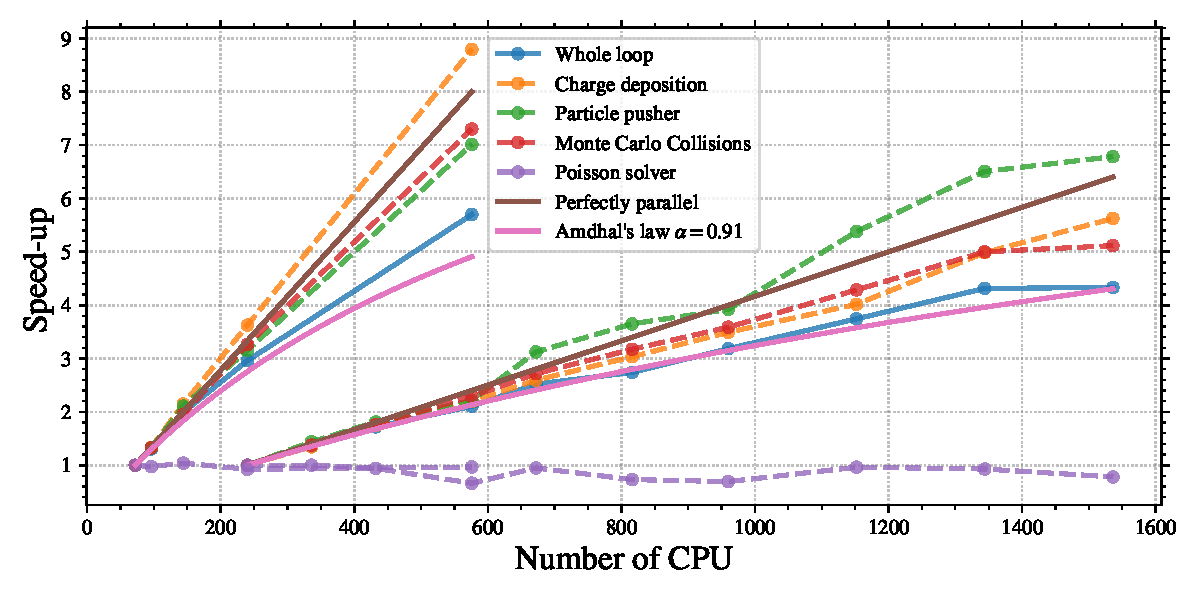
\includegraphics[width=\textwidth]{StrongScalingOccigen_speedup.pdf}
  \caption{Strong scalability profile of \LPPic with a small and a large job on the Cluster Occigen (CINES). In addition to the overall performance, the profiles of the main sub-functions of the \ac{PIC} loops are given. }
  \label{fig-strongperfo}
\end{figure}


We can see that the overall performance of the code is very good, as it scale as if it is parallelized at 91\% from Amdahl's law.
Most of the sub-functions are much better, but the Poisson solver does not scale at all.
Is is due to the size of the chunk of domain of each CPU, which are too small.
A way to improve the performances of \LPPic would be to use an hybridization of the parallelization with the shared memory openMP library.
But the current performance is acceptable, as the typical simulation case presented here runs in around one week (7 days) on 360 CPUs.

\vspace{1em}

The development of the  simulation code \LPPic started in 2015 by Vivien Croes.
I joined the development with Romain Lucken in 2016, and Thomas Charoy started in 2017.
Because of the number of contributors, and our relative experience in Fortran, we quickly set a Continues Integration (CI) pipeline on a self hosted server using Teamcity.
This allows a systematic verification of the modification by the mean of unit, mezzanine and integration tests \citep{turner2016}.

The validation of the code is done using the Benchmark of \citet{turner2013}.
While it allows to validate a significant part of the \ac{PIC} code, it is not magnetized and only in \ac{1D}.
Unfortunately, this is the only Benchmark available.
Hence, the comparison of several codes on a \ac{2D} magnetized  has been conducted by Thomas Charoy in order to create a new Benchmark to validate such simulation codes.


Since 2015, \LPPic has grown to 23000 lines of code, has been used on more than 5 different clusters of various architectures, and has been used to produce several publications \citep{croes2017a,croes2018,tavant2018,tavant2019,lucken2018,lucken2019}.
